\documentclass[11pt]{beamer}
\usepackage[utf8]{inputenc}
\usepackage[T1]{fontenc}
\usepackage{lmodern}
\usepackage[french]{babel}
\usepackage{graphicx}
\usepackage{csvsimple}
\usepackage{tikz}

\usetheme[block=fill,progressbar=frametitle]{metropolis}


\begin{document}
	\author{François-Xavier Jollois}
	\title{A python library to manage ADCP big data}
	\subtitle{Starting joint work with Intechmer}
	%\logo{}
	\institute{diNo -- LIPADE -- Université de Paris}
	\date{May 6th, 2021}
	%\subject{}
	%\setbeamercovered{transparent}
	%\setbeamertemplate{navigation symbols}{}
	\begin{frame}[plain]
		\maketitle
	\end{frame}
	
	\begin{frame}
		\frametitle{Résumé}
		% Les Acoustic Doppler Current Profiler (ADCP) sont des appareils initialement développés pour mesurer les courants d'eau sur la verticale. Les cadences de mesures encore très récemment inférieures à 2 Hz atteignent maintenant 16 Hz, voir 64 Hz pour les prochaines générations. De plus, ces appareils permettent maintenant des mesures simultanées en plusieurs points de la hauteur d'eau. Ces progrès technologiques impliquent d'une part des volumes de données numériques de plus en plus importants. D'autre part, la gamme des conditions d’utilisation des appareils est élargie. Les outils logiciels disponibles pour le traitement et l’analyse des données ADCP, n’ont pas pris en compte, pour la plupart (qu’ils soient propriétaires ou non), le fait d’avoir à gérer des gros volumes de données. Pour permettre une gestion et une analyse des gros volumes de données générés par les plus récents d’appareils de mesure de type ADCP, nous proposons de développer une nouvelle bibliothèque python de calcul.
		
		
		Acoustic Doppler Current Profiler (ADCP) are devices initially developed to measure vertical water currents. The measurement rates still very recently below 2 Hz now reach 16 Hz, or even 64 Hz for the next generations. In addition, these devices now allow simultaneous measurements at several points of the water level. These technological advances involve, on the one hand, increasingly large volumes of digital data. On the other hand, the range of conditions of use of the devices is widened. The software tools available for processing and analyzing ADCP data, for the most part (whether proprietary or not), have not taken into account having to manage large volumes of data. To allow management and analysis of the large volumes of data generated by the most recent ADCP type measuring devices, we are proposing to develop a new python calculation library.
		
	\end{frame}

% What is an ADCP ?
% Why use it ?
% What is complicated to handle these data ?
% What we want to propose
% Our work (in progress)

	\begin{frame}{Outline}
		\tableofcontents
	\end{frame}

	\section{What is an ADCP ?}
	\begin{frame}{\secname}
		
		\begin{definition}
			\textbf{Acoustic Doppler Current Profiler} are devices initially developed to measure vertical water currents velocities, based on \emph{Doppler effect}
		\end{definition}
	
		\begin{center}
			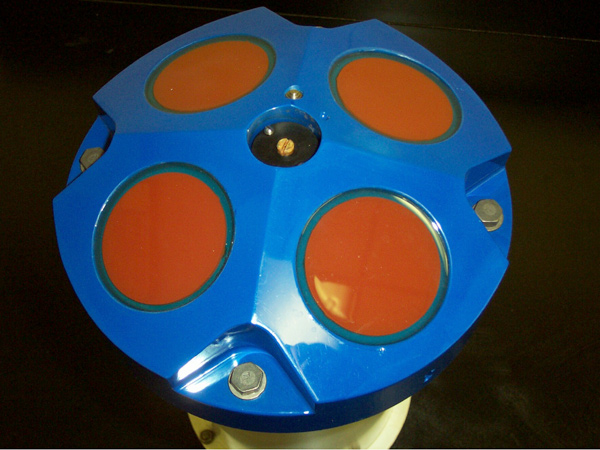
\includegraphics[scale=.25]{Adcp_600}
			%Source: \url{https://en.wikipedia.org/wiki/Acoustic_Doppler_current_profiler}
		\end{center}
	\end{frame}

	\begin{frame}{How ADCP works ?}
		
		\begin{tikzpicture}[scale=.1]
			\draw [black,fill=gray!80] (0,-40) rectangle (3,-39);
			\draw [thick] (-10,-40) -- (50,-40);
			\draw [blue,thick,domain=-10:50,samples=200] plot (\x, {sin(\x r)});
			\fill [black] (1.5,-39) -- (1,-38) -- (2,-38) -- cycle;
			%\draw [red,fill=gray!50,thick] (0.8,-29.8) rectangle (2.2,-31.2);
			\foreach \y in {-1,-2,...,-36} \draw [color=gray!80,densely dotted] (-5,\y) -- (10,\y);
			\draw[rotate=-2,shift={(2, 0)}] (1,-37) grid (2,0);
			\draw[rotate=2,shift={(-2, 0)}] (1, -37) grid (2, 0);

			\node (ping) at (0,10) {Ping};
			\node (ground) at (50,-43) {Ground};
			\node (water) at (50,3) {Sea surface};	
			\node (adcp) at (1.5,-43) {ADCP};
			\node (beam) at (-15,-35) {Beams};
			
			\node (cell) at (20,-20) {Cell};
			\node (bin) at (20,-27.5) {Bin};
			\node[draw,circle] (bin_t) at (2.5,-30.5) {};
			
			%\draw[->] (ping) -- (1.5,0);
			\draw[->] (beam) -- (1,-38);
			\draw[->] (cell) -- (10,-20.5);
			\draw[->] (bin) -- (bin_t);
		\end{tikzpicture}
	
	\end{frame}

	\begin{frame}{What are the data collected ?}
		\begin{block}{Global data}
			ADCP type (especially number of beams), Position (on the ground or under a boat), Number of cells (and size), Blancking (device near blind area) 
		\end{block}
		\begin{block}{Ping specific data}
			Timestamp, ADCP rotation (on 3 axes), ENU position (if moving), Temperature, Salinity, Speed of sound, Depth
		\end{block}
		\begin{block}{Bin specifica data}
			Velocity, correlation (quality of measure), intensity (of measure)
		\end{block}
	\end{frame}

	\section{For which purpose ?}
	\begin{frame}{\secname}
		\begin{itemize}
			\item Estimation of the water current
			\item Development of Marine Renewable Energy (i.e. tidal turbine)
			\item Alderney Race (\textit{Raz Blanchard})\footnote{\url{http://www.wikimanche.fr/Raz_Blanchard}}
				\begin{itemize}
					\item One of the most powerful current in Europe
					\item Current velocity (arrows) up to 5 m/s (12 knots)
				\end{itemize}
		\end{itemize}
		\begin{center}
			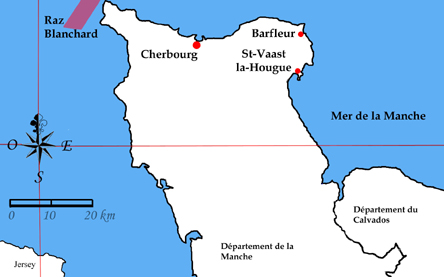
\includegraphics[scale=.5]{raz_blanchard}
		\end{center}
	\end{frame}

	\section{What is complicated to handle these data ?}
	\begin{frame}{\secname}
		\begin{itemize}
			\item Raw binary files
			\item Data quality should be estimated
			\item Possible huge amount of data
			\item Data (after transformations) are vectors: velocity and direction
		\end{itemize}
	\end{frame}

	\begin{frame}{Raw binary files}
		Raw binary files
		\begin{itemize}
			\item Files are pure binary that we need to decode
			\item Each ping is defined by a specific starting and ending binary sequence
			\item Each manufacturer has its own binary format
		\end{itemize}
	
		Data quality
		\begin{itemize}
			\item Measurements are subject to defects
			\item Shoaling fish, water infiltration, lost device\ldots
		\end{itemize}
	\end{frame}

	\begin{frame}{How huge are the data collected ?}
		\begin{itemize}
			\item Time series: data are collected during a given period (from some hours to several weeks or months)
			\item Frequency of ping: 2Hz to 16Hz, even more in the next years
			\item Multiple beams: 3 or 4, even more in the next years
			\item Multiple cells: usual size of cells is 1 meter (even smaller in the next years), so it can be 30 to 40 cells in our case
		\end{itemize}
	
		\begin{block}{For instance}
			2 weeks at 8Hz with 5 beams on 40 cells $\rightarrow$  ~1.9 G bins
		\end{block}
	\end{frame}

	\begin{frame}{Data are vectors}
		\begin{itemize}
			\item For each ping, for each cell, 
		\end{itemize}
		\begin{tikzpicture}[scale=.2]
			\draw[->] (0,0,0) -- (50,0,0) node {Time};
			\csvreader[ head to column names]%
			{vectors.csv}{}{%
				\draw[->] (\xo, \zo, \yo) -- (\x, \z, \y);
			}
		\end{tikzpicture}
	\end{frame}

	\begin{frame}{Data need to be reconstructed}
		\begin{itemize}
			\item Velocity in a bin : numerical value indicating if the current is going to the beam cell (positive) or not (negative) $\rightarrow$ vertically measure
			\item Combination of values in the different beams to get the current measure in each cell
			\item Device could rotate due to the current
		\end{itemize}
	\end{frame}

	\section{What we want to propose ?}
	\begin{frame}{\secname}
		A python library to manage ADCP files, using parallel processing
		\begin{itemize}
			\item Binary files transformation into NetCDF files
			\item Coordinates transformation (if needed)
			\item Compute classical values on NetCDF files
			\item Visualisation of NetCDF files
			\item Analysis such as
				\begin{itemize}
					\item Detection of optimal sliding window for current average
					\item Detection of current turbulences
				\end{itemize}
		\end{itemize}
	\end{frame}

	\section{Our work (in progress)}
	\begin{frame}{\secname}
		\begin{itemize}
			
			\item 
		\end{itemize}
	\end{frame}

	\section{Conclusion}
	\begin{frame}{\secname}
		content
	\end{frame}

\end{document}